% SC4064 --- Chapter 1: GPU Architecture, SIMT and the CPU--GPU Divide (0->100 ground-up)
\chapter{Introduction: GPU Architecture, SIMT and the CPU--GPU Divide}
\label{ch:intro-gpu}
\sloppy

\begin{quote}
\emph{``The GPU is not a faster CPU---it is a different philosophy of computing.''} A CPU makes one runner very fast; a GPU fields a stadium of slower runners and wins by sheer throughput. This chapter explains why that trade exists, how the hardware expresses it, and when each philosophy wins.
\end{quote}

\noindent\fbox{\parbox{\dimexpr\linewidth-2\fboxsep-2\fboxrule}{%
\textbf{From zero: no GPU or parallel background assumed.} We start from a single sequential program and ask what happens when we throw thousands of tiny workers at the same problem. Every term---core, SM, warp, SIMT---is defined on first use, picture first, then formal.}}
\vspace{0.4em}

\section*{Learning Outcomes}
After this chapter you will be able to:
\begin{enumerate}[label=(L\arabic*)]
    \item contrast latency-optimised (CPU) and throughput-optimised (GPU) design goals;
    \item describe the GPU hierarchy (device $\to$ SM $\to$ warp $\to$ thread) and the role of each level;
    \item define SIMT execution and explain warp-level lockstep, divergence and masking;
    \item compare SIMD, SIMT and MIMD with examples and state where each excels;
    \item place a workload on the Roofline and argue CPU versus GPU suitability.
\end{enumerate}

% ============================================================
\section{Why GPUs Exist: Two Philosophies of Speed}
\label{sec:why-gpu}
\paragraph{Intuition.} Imagine delivering 10\,000 letters. A CPU is a sports car with a superb navigator: it delivers one letter blazingly fast, with branch prediction guessing turns and a huge cache remembering the map. A GPU is a fleet of 10\,000 bicycles that all leave together on the same route: each is slow alone, but the fleet moves the whole pile in one wave. If your job is one urgent letter, take the car. If it is the whole pile, take the fleet.

A CPU optimises \emph{latency}: minimise time for a single task. It spends transistors on large caches, deep branch predictors, out-of-order scheduling and low-latency control. A GPU optimises \emph{throughput}: maximise tasks per second. It spends transistors on many simple cores, wide memory buses, and hardware that swaps warps instantly to hide stalls. Neither is universally better; they are Pareto-optimal at opposite ends.

\begin{figure}[h]\centering
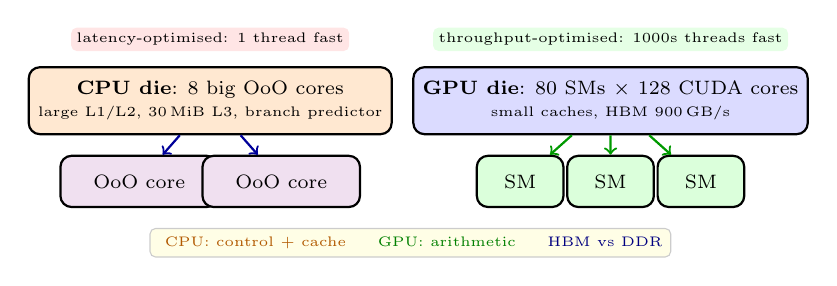
\begin{tikzpicture}[scale=0.82, every node/.style={font=\scriptsize},
  block/.style={draw, thick, rounded corners=4pt, align=center, minimum height=0.85cm}]
\node[block, fill=orange!18, minimum width=3.8cm] (cpu-die) at (0,1.6) {\textbf{CPU die}: 8 big OoO cores\\{\tiny large L1/L2, 30\,MiB L3, branch predictor}};
\node[block, fill=blue!14, minimum width=3.8cm] (gpu-die) at (6.2,1.6) {\textbf{GPU die}: 80 SMs $\times$ 128 CUDA cores\\{\tiny small caches, HBM 900\,GB/s}};
\node[block, fill=violet!12, minimum width=2.0cm, minimum height=0.65cm] (cpu-c) at (-1.1,0.35) {OoO core};
\node[block, fill=violet!12, minimum width=2.0cm, minimum height=0.65cm] (cpu-c2) at (1.1,0.35) {OoO core};
\node[block, fill=green!14, minimum width=1.1cm, minimum height=0.65cm] (sm1) at (4.8,0.35) {SM};
\node[block, fill=green!14, minimum width=1.1cm, minimum height=0.65cm] (sm2) at (6.2,0.35) {SM};
\node[block, fill=green!14, minimum width=1.1cm, minimum height=0.65cm] (sm3) at (7.6,0.35) {SM};
\node[font=\tiny, fill=red!10, rounded corners=2pt, inner sep=2pt] at (0,2.55) {latency-optimised: 1 thread fast};
\node[font=\tiny, fill=green!10, rounded corners=2pt, inner sep=2pt] at (6.2,2.55) {throughput-optimised: 1000s threads fast};
\draw[->, thick, blue!60!black] (cpu-die) -- (cpu-c);
\draw[->, thick, blue!60!black] (cpu-die) -- (cpu-c2);
\draw[->, thick, green!60!black] (gpu-die) -- (sm1);
\draw[->, thick, green!60!black] (gpu-die) -- (sm2);
\draw[->, thick, green!60!black] (gpu-die) -- (sm3);
\node[font=\tiny, align=left, fill=yellow!10, draw=gray!40, rounded corners=2pt, inner sep=3pt] at (3.1,-0.60) {\textcolor{orange!70!black}{$\blacksquare$ CPU: control + cache} \quad \textcolor{green!50!black}{$\blacksquare$ GPU: arithmetic} \quad \textcolor{blue!50!black}{$\blacksquare$ HBM vs DDR}};
\end{tikzpicture}
\caption{CPU versus GPU transistor budget: CPUs buy latency (caches, predictors, OoO), GPUs buy throughput (many simple datapaths and wide HBM).}
\label{fig:cpu-vs-gpu}
\end{figure}

The same trade appears on the Roofline: a kernel with low arithmetic intensity (bytes per flop) is memory-bound and needs bandwidth (GPU wins); a kernel with branches and irregular dependencies is latency-bound (CPU wins). Knowing the workload's Roofline point is the first step in choosing a device.

% ============================================================
\section{GPU Anatomy: From Device to Thread}
\label{sec:anatomy}
A modern NVIDIA GPU (Ampere/Hopper) is a three-level hierarchy.

\paragraph{Device.} The whole chip: 60--144 \emph{Streaming Multiprocessors (SMs)}, a shared L2 (40--50\,MiB), display/media engines, and high-bandwidth memory (HBM2e/HBM3, 900\,GB/s--3\,TB/s). The host CPU launches work via PCIe/NVLink.

\paragraph{Streaming Multiprocessor (SM).} The workhorse. Each SM holds 64--128 CUDA cores (FP32), 4 warp schedulers, a large register file (64K $\times$ 32-bit), L1/shared memory (128--228\,KiB configurable), and special units (tensor cores, RT cores, load/store). An SM executes warps, not individual threads, and can keep 32--64 warps resident to hide latency.

\paragraph{Warp and thread.} A \emph{warp} is 32 threads that advance in lockstep (SIMT). A \emph{thread} is the smallest unit: one program counter plus private registers. Threads are grouped by the programmer into \emph{blocks} (up to 1024 threads), blocks into a \emph{grid}; the hardware maps blocks to SMs and warps within a block to schedulers.

\begin{figure}[h]\centering
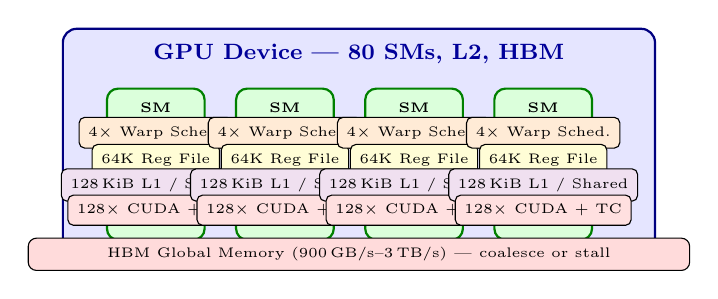
\begin{tikzpicture}[scale=0.80, every node/.style={font=\scriptsize}]
\draw[fill=blue!10, draw=blue!50!black, thick, rounded corners=5pt] (-0.4,-2.1) rectangle (9.0,1.7);
\node[font=\footnotesize\bfseries, text=blue!60!black] at (4.3,1.30) {GPU Device --- 80 SMs, L2, HBM};
\foreach \x in {0.30,2.35,4.40,6.45} {
  \draw[fill=green!14, draw=green!50!black, thick, rounded corners=4pt] (\x,-1.65) rectangle (\x+1.55,0.75);
  \node[font=\tiny\bfseries] at (\x+0.775,0.45) {SM};
  \node[draw, fill=orange!16, rounded corners=2pt, minimum width=1.15cm, minimum height=0.35cm, font=\tiny] at (\x+0.775,0.05) {4$\times$ Warp Sched.};
  \node[draw, fill=yellow!16, rounded corners=2pt, minimum width=1.20cm, minimum height=0.32cm, font=\tiny] at (\x+0.775,-0.38) {64K Reg File};
  \node[draw, fill=violet!12, rounded corners=2pt, minimum width=1.20cm, minimum height=0.32cm, font=\tiny] at (\x+0.775,-0.78) {128\,KiB L1 / Shared};
  \node[draw, fill=red!12, rounded corners=2pt, minimum width=1.20cm, minimum height=0.30cm, font=\tiny] at (\x+0.775,-1.18) {128$\times$ CUDA + TC};
}
\node[draw, fill=red!14, rounded corners=3pt, minimum width=8.4cm, minimum height=0.40cm, font=\tiny] at (4.3,-1.88) {HBM Global Memory (900\,GB/s--3\,TB/s) --- coalesce or stall};
\end{tikzpicture}
\caption{GPU SM hierarchy: a device of many SMs, each with warp schedulers, a large register file, configurable L1/shared, and CUDA/tensor cores. Keeping many warps resident hides latency.}
\label{fig:gpu-sm}
\end{figure}

\begin{definition}[SM, warp, thread]
An \emph{SM} is a self-contained processor that executes warps. A \emph{warp} is 32 threads sharing a program counter and advancing in SIMT lockstep. A \emph{thread} is one SIMT lane with private registers; divergence within a warp is serialised with masking.
\end{definition}

% ============================================================
\section{SIMT Execution and Divergence}
\label{sec:simt}
\emph{SIMD} (single instruction, multiple data) has one instruction operating on a vector of data in lockstep. \emph{SIMT} looks similar but is subtly different: each thread has its own program counter and can, in principle, diverge. Hardware makes divergence correct but slow: when threads of a warp take different branches, the warp executes each path sequentially with inactive lanes masked off.

\begin{figure}[h]\centering
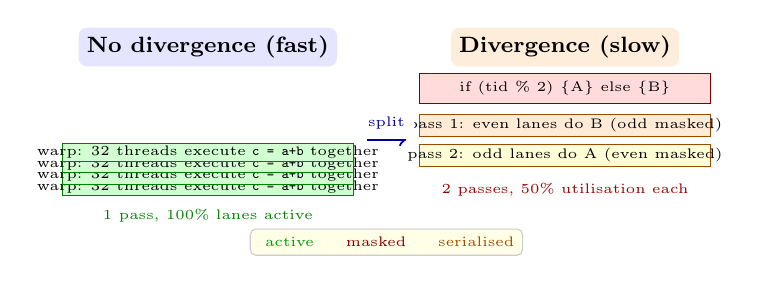
\begin{tikzpicture}[scale=0.84, every node/.style={font=\scriptsize}]
\node[font=\footnotesize\bfseries, fill=blue!10, rounded corners=3pt, inner sep=3pt] at (2.2,2.6) {No divergence (fast)};
\foreach \i in {0,0.5,1.0,1.5} {
  \draw[fill=green!18, draw=green!50!black] (0,\i*0.35+0.35) rectangle (4.4,\i*0.35+0.62);
  \node[font=\tiny] at (2.2,\i*0.35+0.485) {warp: 32 threads execute \texttt{c = a+b} together};
}
\node[font=\tiny, text=green!50!black] at (2.2,0.05) {1 pass, 100\% lanes active};

\node[font=\footnotesize\bfseries, fill=orange!14, rounded corners=3pt, inner sep=3pt] at (7.6,2.6) {Divergence (slow)};
\draw[fill=red!14, draw=red!50!black] (5.4,1.75) rectangle (9.8,2.20);
\node[font=\tiny, align=center] at (7.6,1.98) {if (tid \% 2) \{A\} else \{B\}};
\draw[fill=orange!16, draw=orange!60!black] (5.4,1.25) rectangle (9.8,1.58);
\node[font=\tiny] at (7.6,1.415) {pass 1: even lanes do B (odd masked)};
\draw[fill=yellow!16, draw=orange!60!black] (5.4,0.80) rectangle (9.8,1.13);
\node[font=\tiny] at (7.6,0.965) {pass 2: odd lanes do A (even masked)};
\node[font=\tiny, text=red!60!black] at (7.6,0.45) {2 passes, 50\% utilisation each};
\draw[->, thick, blue!60!black] (4.6,1.2) -- (5.2,1.2) node[midway, above, font=\tiny, fill=white] {split};
\node[font=\tiny, fill=yellow!10, draw=gray!40, rounded corners=2pt, inner sep=3pt] at (4.9,-0.35) {\textcolor{green!60!black}{$\blacksquare$ active} \quad \textcolor{red!50!black}{$\blacksquare$ masked} \quad \textcolor{orange!60!black}{$\blacksquare$ serialised}};
\end{tikzpicture}
\caption{SIMT divergence: a warp with no divergence finishes in one pass; a branch that splits the warp executes both paths sequentially with masking, halving throughput.}
\label{fig:simt-diverge}
\end{figure}

The rule of thumb is simple: keep warps \emph{converged}. Data-dependent branches where all 32 threads agree are free; branches that split a warp cost proportionally to the number of distinct paths. Sorting or tiling work so that threads in a warp follow the same path is a core GPU optimisation (Ch.~4).

\begin{example}[Divergence cost]
A kernel with \texttt{if(data[tid] > 0) \{ heavyA(); \} else \{ heavyB(); \}} and random data splits every warp roughly 50/50, doubling runtime. If data is sorted so warps are homogeneous (all-positive vs.\ all-negative blocks), each warp takes one path and runtime returns to near-optimal.
\end{example}

\begin{lstlisting}[language=C++, caption={CPU sequential baseline vs.\ GPU SIMT kernel: same maths, different execution philosophy.}, label={lst:cpu-vs-gpu}]
// CPU: one fast thread loops sequentially
void cpuVecAdd(float *a, float *b, float *c, int n){
    for(int i=0;i<n;i++) c[i] = a[i] + b[i]; // latency-optimised core
}
// GPU: thousands of thin threads, one element each, in SIMT lockstep
__global__ void gpuVecAdd(float *a, float *b, float *c, int n){
    int i = blockIdx.x * blockDim.x + threadIdx.x; // global id (Ch.2)
    if(i < n) c[i] = a[i] + b[i]; // warp executes together when converged
}
\end{lstlisting}

\begin{lstlisting}[language=Python, caption={Roofline intuition: which device for which kernel?}, label={lst:roofline-intro}]
# Roofline: attainable = min(peak_flops, bandwidth * intensity)
peak_cpu, bw_cpu = 1e12, 100e9    # 1 TFLOP, 100 GB/s
peak_gpu, bw_gpu = 15e12, 900e9   # 15 TFLOP, 900 GB/s
for name, ops, bytes_ in [("saxpy",2,12),("matmul",2,0.25),("branchy",1,8)]:
    intensity = ops/bytes_        # FLOPs per byte
    cpu = min(peak_cpu, bw_cpu*intensity)
    gpu = min(peak_gpu, bw_gpu*intensity)
    print(f"{name:8s} I={intensity:.2f}  CPU {cpu/1e12:.1f} TF  GPU {gpu/1e12:.1f} TF")
# saxpy (low I) is bandwidth-bound -> GPU wins on BW
# matmul (high I) is compute-bound -> GPU wins on peak
# branchy irregular -> CPU wins despite lower peak (divergence)
\end{lstlisting}

% ============================================================
\section{A Worked Comparison: Latency vs.\ Throughput in Numbers}
\label{sec:worked-compare}
Take vector addition of $n=1\,048\,576$ floats. A 3.5\,GHz CPU core with AVX-512 does 16 FLOPs/cycle $\Rightarrow$ 56\,GFLOP/s and streams at $\sim$50\,GB/s from DDR. A mid-range GPU has 30 SMs $\times$ 128 cores at 1.5\,GHz $\approx$ 11\,TFLOP/s and 600\,GB/s from HBM. The kernel intensity is $I=2\,\text{FLOPs}/12\,\text{bytes}=0.167$ FLOP/B (two loads, one store, one add).

Roofline attainable performance is $\min(\text{peak}, \text{BW}\times I)$. On CPU: $\min(56, 50\times0.167=8.35)=8.35$\,GFLOP/s. On GPU: $\min(11000, 600\times0.167=100)=100$\,GFLOP/s, a $12\times$ advantage from bandwidth alone. Yet if the kernel were a binary search with unpredictable branches, SIMT divergence would serialize warps and the CPU's predictor and low latency would dominate despite lower peak.

\begin{remark}[The golden rule of GPU computing]
GPUs reward \emph{uniform, independent, arithmetic-heavy} work. Uniform means warps agree on branches; independent means threads need little cross-talk; arithmetic-heavy (or bandwidth-heavy with coalescing, Ch.~3) keeps the massive datapath busy. Violate any leg and the advantage collapses---that is why CPUs still run operating systems, databases and compilers.
\end{remark}

A second lens is \emph{Little's Law} for latency hiding. If global memory latency is $L=400$ cycles and each warp does $W=4$ cycles of math before needing data, one warp keeps the SM busy $W/(W+L)\approx1\%$ of the time. With $N$ warps the SM stays busy $\min(1, N\cdot W/(W+L))$. Solving $N\ge (W+L)/W\approx101$ warps for $100\%$ utilisation shows why GPUs need \emph{occupancy}: many resident warps cover the gap one warp leaves while waiting.

\begin{definition}[Arithmetic intensity and Roofline]
\emph{Arithmetic intensity} $I=$ FLOPs / bytes moved from DRAM. The \emph{Roofline model} bounds attainable throughput as $\min(\text{peak FLOP/s}, \text{peak BW}\times I)$. The knee where the two terms equal is the \emph{ridge point} $I^*=\text{peak}/\text{BW}$; left is memory-bound, right is compute-bound.
\end{definition}

\paragraph{What this means for you.} Before writing a kernel, ask: is my problem \emph{data-parallel} (same operation on many elements) or \emph{task-parallel} (different operations)? Data-parallel maps to SIMT; task-parallel maps to MIMD (CPU threads or multi-GPU). Within data-parallel, ask: will warps diverge? Profile a histogram of branch outcomes per warp, not per thread. If divergence is high, consider data layout transforms (structure-of-arrays, sorting keys) or algorithmic changes (branchless selects). Finally, estimate intensity early: count FLOPs and bytes in the inner loop. If $I\ll I^*$, optimise memory (coalescing, shared tiling, Ch.~3) before touching arithmetic.

\begin{example}[Choosing the device]
Image blur (3$\times$3 stencil): each output pixel needs 9 multiplies and a handful of loads; warps are fully converged and accesses are regular---ideal GPU work, $8$--$15\times$ faster than a multi-core CPU. Binary search in a sorted array: each thread follows a different path length, divergence is maximal and locality is poor---CPU wins by $5$--$20\times$. The deciding factor is not FLOP count but \emph{uniformity of control} and \emph{regularity of memory}.
\end{example}

% ============================================================
\section{Exercises}
\label{sec:ch01-exercises}
\begin{enumerate}[label=E1.\arabic*, leftmargin=*, itemsep=0.6em]
    \item \textbf{CPU vs.\ GPU budgeting.} A chip has 10\,B transistors. A CPU core + its cache costs 1\,B, an SM costs 0.2\,B. How many cores/SMs per design? For a perfectly parallel kernel with 10\,000 independent elements, estimate ideal speedup of the GPU design assuming one SM matches one core's throughput on one element. When does the CPU win?
    \item \textbf{SIMT vs.\ SIMD vs.\ MIMD.} Define each and give one real example (e.g., SSE, NVIDIA warp, multicore cluster). Why can SIMT handle \texttt{if} divergence (with masking) while pure SIMD cannot handle arbitrary control flow efficiently?
    \item \textbf{Warp divergence arithmetic.} A kernel branch splits warps 25/75 on average (25\% lanes go path A, 75\% path B, paths cost equal time $T$). What is the warp execution time versus a converged warp? If you sort data so warps become 100/0 or 0/100, what is the new time and speedup?
    \item \textbf{SM occupancy intuition.} An SM supports 2048 threads and 64 warps. Block size is 128 threads (4 warps). How many blocks fit per SM thread-wise? Why might fewer actually fit due to registers or shared memory? No exact numbers needed---explain the limiting idea.
    \item \textbf{Roofline placement.} A kernel does 5 FLOPs per 4-byte element (intensity $1.25$ FLOP/B). CPU ridge point is 10 FLOP/B, GPU ridge is 16.7 FLOP/B (15\,TF/900\,GB/s). Is it memory or compute bound on each? Which device gives higher attainable performance and by what factor?
\end{enumerate}

\paragraph{Looking ahead.} Chapters~2--4 turn this picture into practice. Chapter~2 gives you the programming model that maps threads to SMs; Chapter~3 shows how memory layout makes or breaks the Roofline you just learned to read; Chapter~4 teaches you to measure occupancy and overlap and to know when the GPU is truly busy. Keep the two-philosophies figure in mind---every optimisation is about pushing a workload toward the throughput peak or recognising when latency matters more.

\begin{remark}[How to read the rest of this book]
Each chapter follows the same arc: intuition and picture $\to$ formal definition $\to$ worked example with numbers $\to$ runnable code you can compile with \texttt{nvcc -arch=sm\_80} $\to$ exercises. Run every listing; change a parameter (block size, data layout) and re-measure. The intuition tells you what to expect; the measurement tells you whether you got it. That loop is the core skill of GPU programming.
\end{remark}

\begin{example}[Mental model check]
Before moving on, test your model: a kernel launches 1\,M threads each doing \texttt{c[i]=a[i]+b[i]}. (a) How many warps? (b) If one SM holds 64 warps, how many wavefronts to cover the grid on a 40-SM GPU? (c) Where is the bottleneck---ALUs or memory? Answers: (a) $1\,048\,576/32=32\,768$ warps. (b) $32\,768/(40\times64)\approx12.8$ waves. (c) Memory---each thread moves 12 bytes for 1 FLOP, so bandwidth dominates. This back-of-envelope predicts the Roofline result.
\end{example}

\paragraph{Checkpoint.} You should now picture a GPU as a grid of SMs each juggling dozens of warps, with warps as the scheduling quantum and threads as lanes. The next chapter turns that picture into code: how you name threads, group them, and launch a kernel that the hardware maps to this hierarchy.

\smallskip

% ============================================================
\section*{Chapter Notes}
Lamport's definition and early GPU history are covered in Kirk \& Hwu, \emph{Programming Massively Parallel Processors} (4th ed., 2022, Ch.~1--2) and Hennessy \& Patterson, \emph{Computer Architecture: A Quantitative Approach} (6th ed., App.~A on GPUs). SIMT terminology originates with NVIDIA's Tesla architecture (Lindholm et~al., 2008). Roofline: Williams et~al., CACM 2009. CUDA C++ Programming Guide (NVIDIA, v12.x) \S1--2 is the authoritative device/SM description; verify SM counts and HBM figures against the specific GPU you target (A100/H100 tables).
% End of Chapter 1
